\section{Clustering Algorithms}
\label{clustering-algorithms}


\subsection{k-center}
\label{k-center}

\subsubsection{General}
The k-center clustering is a NP-hard problem. Because it is very likely that there never will be efficient algorithms to solve NP-hard problems, you need to resort to approximation algorithms.
For example, there is a greedy algorithm by \textcite[]{Gonzalez1985ClusteringDistance} which can solve our problems.

This k-center algorithm consists of a parameter $k$, which defines the number of center points, and a set of center points $C$, where $c_{1},...,c_{k}$ are the so-called centers. \autocite[]{Kleindessner2019FairSummarization}
The greedy strategy by \textcite[]{Gonzalez1985ClusteringDistance} picks an arbitrary element of the data set as the first center point $c_{1}$, calculates the distance for every point in the data set and picks the point with the highest distance as next center point $c_{2}$. This process will be continued until k center points are found.

\subsubsection{Fairness}

The fair variant of \textcite[]{Kleindessner2019FairSummarization} allows for the user to specify a subset $C_{0} \subseteq S$ that has to be included in the set of centers.

\textcite[]{Chierichetti2018} uses the concept of \nameref{fairlets}. In his work, he has two different approaches for k-center: the $(1,1)$-fairlets and the $(1,t')$-fairlets.

The $(1,1)$ approach, that they also called "warmup", should be an example for a perfectly balanced clustering. \autocite[6]{Chierichetti2018}

In the approach with the $(1,t')$-fairlets, they use a clustering with balance $t < 1$ instead, so it is assumed that $t = \frac{1}{t'}$, where $t'$ is an integer value $> 1$. \autocite[6]{Chierichetti2018}


\subsection{k-means \& k-median}
\label{k-means}
\label{k-median}

\subsubsection{General}

"The global $k$-means clustering algorithm" was introduced by \textcite[]{Likas2003}. They explain that their algorithm "is an incremental approach to clustering that dynamically adds one cluster center at a time through a deterministic global search procedure consisting of $N$ (with $N$ being the size of the data set) executions of the $k$-means algorithm from suitable initial positions." \autocite[1]{Likas2003}

As \textcite[]{Jain1988} said, k-median is basically an extension for the k-means algorithm with the only difference, that it uses the median instead of the mean in each dimension.

In detail, \textcite[2]{Likas2003} explain the $k$-means algorithm with a given "data set $X = \{x_{1},...,x_{N}\},x_{n} \in \mathbb{R}^d$". Then they try to partition "this data set into $M$ disjoint subsets (clusters) $C_{1},...,C_{M}$" to aim the so-called $M$-clustering problem, "such that a clustering criterion is optimized." They add,that "The most widely used clustering criterion is the sum of the squared Euclidean distances between each data point $x_{i}$ and the centroid $m_{k}$ (cluster center) of the subset $C_{k}$ which contains $x_{i}$. This criterion is called clustering error and depends on the cluster centers $m_{1},...,m_{M}$, [...] where $I(X) = 1$ if $X$ is true and $0$ otherwise.

\subsubsection{Fairness}

\textcite[]{Chierichetti2018}, who had a look at the $k$-median clustering algorithm, have put forward the theorem that "the algorithm that first finds fairlets and then clusters them is a $(2 + \sqrt{3} + \epsilon)$-approximation for the (1, $k$)-fair median problem." This can be also modified for approximations like $(t' + 1 + \sqrt{3} + \epsilon)$ for the $(\frac{1}{t'}, k)$-fair median problem. \autocite[9]{Chierichetti2018}

For the k-means clustering algorithm, \textcite[]{Schmidt2018} wanted to get another solution, because they discovered that "previous algorithms for fair clustering do not scale well." So they came up with a solution of "coresets for fair clustering problems", especially for the $k$-means algorithm, where they are showing how to model and how to compute them. These coresets should be there to be able to drastically reduce the size of the input data. They have proven that these coresets can also be easily put together and they also show the possibility of computation in a streaming environment. \autocite[1]{Schmidt2018} 


\subsection{Spectral Clustering}
\label{spectral-clustering}

\subsubsection{General}

When it comes to the spectral clustering method for cluster analysis, the work of \textcite[]{VonLuxburg2007}  "A Tutorial on Spectral Clustering" is a good place to start. It defines this method of clustering as follows:

\begin{quote}
"Compared to the “traditional algorithms” such as k-means or single linkage, spectral clustering has many fundamental advantages. Results obtained by spectral clustering often outperform the traditional approaches, spectral clustering is very simple to implement and can be solved efficiently by standard linear algebra methods."

\autocite[1]{VonLuxburg2007}
\end{quote}

Spectral clustering is based on so-called similarity graphs. These show similarities between different data points in an undirected graph $G = (V,E)$. The data is divided into groups: data points in the same group are similar, points in different groups are different. \autocite[2]{VonLuxburg2007}

As \textcite[2]{Kleindessner2019} summarize for creating an algorithm for unnormalized spectral clustering, a weighted adjacency matrix is calculated from the similarity graph, and subsequently the Laplacian matrix of it. Then the $k$ smallest eigenvalues of the Laplacian matrix and the corresponding orthonormal eigenvectors are computed. A $k$-means clustering is then applied to this.

While \textcite[]{Kleindessner2019} mainly deal with unnormalized spectral clustering, there are two known variants of normalized spectral clustering by \textcite[]{Shi2000} and \textcite[]{Ng2001}.

\begin{quote}
"The success of spectral clustering is mainly based on the fact that it does not make strong assumptions on the form of the clusters. As opposed to $k$-means, where the resulting clusters form convex sets (or, to be precise, lie in disjoint convex sets of the underlying space), spectral clustering can solve very general problems like intertwined spirals."

\autocite[28]{VonLuxburg2007}
\end{quote}

\subsubsection{Fairness}

In addition to the weighted adjacency matrix, the fair algorithm of \textcite[3]{Kleindessner2019} in spectral clustering requires a group $f^{(s)} \in \{0,1\}^n, s \in [h]$. This allows to compute a fairness matrix which is used instead of the Laplace matrix to get a fair spectral clustering. \autocite[3]{Kleindessner2019}

To be able to better demonstrate this, \textcite[4]{Kleindessner2019} showed a variant of the stochastic block model with 4 blocks of graph data (\ref{fig:kleindessner_variant_sbm}), where points in each group have different properties:
\begin{enumerate}
	\item both points in the same cluster and group.
	\item both points not in the same cluster but in the same group
	\item both points in the same cluster but not in the same group
	\item both points neither in the same cluster, nor in the same group
\end{enumerate}

When you look at \autoref{fig:kleindessner_variant_sbm}, you can see that the clustering $V = C_{1} \dot\cup C_{2}$ is fair, but the clustering $V = V_{1} \dot\cup V_{2}$ would be highly unfair. \autocite[4]{Kleindessner2019}

\begin{figure}
    \centering
    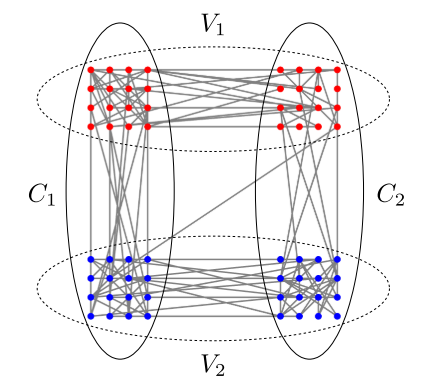
\includegraphics[width=0.9\linewidth]{images/kleindessner_variant_sbm.png}
    \caption{Variant of the Stochastic Block Model of \textcite[4]{Kleindessner2019}}
    \label{fig:kleindessner_variant_sbm}
\end{figure}